\chapter{Policy Gradient Methods}
So far we focused on action-value methods, those methods learned the action-value function $q$ and used it to derive a policy. In this chapter, we will focus on methods that learn the policy directly, without consulting a value, or action-value function. The value function still has an important role as it's often used to learn the policy, however, it is not required for action selection. This class of methods is called policy gradient methods.\\\\
Policy gradient methods can be applied without function approximation. However, in this discussion, we will focus on the function approximation setting, where the policy is expressed as a function of the state $s$ and a vector of parameters $\vect{\theta}$, expressed as $\pi(a|s; \vect{\theta})$.\\\\
We will begin by covering the basics of function approximation, specifically neural networks, which will serve as the foundation for all the algorithms discussed in this chapter. We will then delve into the policy gradient theorem for discrete action spaces and introduce REINFORCE, a Monte Carlo policy gradient algorithm.\\
Our main focus will be on actor-critic methods, which have achieved significant success in various domains, such as playing games like Dota 2 \cite{open-ai-five}, StarCraft II \cite{alphastar, wang2021scc}, Go \cite{alphago-fan}, Minecraft \cite{minecraft-vpt, dreamer-v3} with also applications to language like ChatGPT \cite{instruct-gpt}. We will not provide an exhaustive overview of actor-critic methods, but we will discuss key ones, such as TRPO and PPO. The latter will also be used to in the subsequent chapter to learn to play Briscola.

\section{Function Approximation}
The methods discussed so far represent the action-value function $q(s, a)$ as a table and are thus called tabular methods. These methods have been shown to converge to an optimal policy under certain conditions, such as proper selection of the step-size $\alpha$ and the policy $\epsilon$ parameter. However, tabular methods can be impractical to use in certain scenarios, such as when the state space is extremely large (e.g. in the game of chess) or when the state space is continuous. In these cases, function approximation must be used to represent the value function, action-value function, and policy.\\\\
To keep things clear, we will focus on approximating the value function, denoted as $\hat{v}(s; \vect{w})$, where $\vect{w}$ is a parameter vector. The same ideas can also be applied to the action-value function or the policy. Furthermore, we assume to perform function approximation with neural networks, as they are widely used in practical applications and offer differentiable function approximation \cite{lecun2015deep}, which is a critical requirement for the policy gradient theorem.
Consider the problem of finding the value function corresponding to a policy $\pi$, thus far we implemented the update rule for the value function by moving the value prediction $V(s)$ closer to the return $G_t$, which represents the target:
\begin{equation}
    V(s) = V(s) + \alpha (G_t - V(s))
    \label{eq:tabular-update}
\end{equation}
With function approximation the idea is the same, moving the prediction closer to the target. But instead of updating the value of the table entry $V(s)$ directly, we need to update the parameter vector $\vect{w}$. The way we usually update the parameter vector $\vect{w}$ in neural networks is with gradient descent, that is, we update $\vect{w}$ in the negative direction of the gradient of a loss function $L$.
\begin{equation}
    \vect{w} = \vect{w} - \alpha \nabla_w L(\hat{v}(s; \vect{w}), G_t)
    \label{eq:nn-update}
\end{equation}
The loss function measures how far the value prediction $\hat{v}(s; \vect{w})$ is from the target $G_t$. A natural loss function for learning the value is the \textit{mean squared error loss} denoted as $L_\textrm{MSE}$:
\begin{equation}
    L_\textrm{MSE} = \frac{1}{2}(G_t - \hat{v}(S_t; \vect{w}))^2
    \label{eq:mse}
\end{equation}
The gradient of the loss function \eqref{eq:mse} with respect to $\vect{w}$, can be quickly computed:
\begin{equation}
    \nabla_{w} L_\mathrm{MSE} = \left( \hat{v}(S_t; \vect{w}) - G_t \right) \nabla_w \hat{v}(S_t; \vect{w})
    \label{eq:mse-gradient}
\end{equation}
Where $\nabla_w \hat{v}(s; \vect{w})$ is the gradient of the output of the function with respect to the parameter vector $\vect{w}$ and can be quickly found with automatic differentiation techniques.\\\\
Tabular methods can be viewed as a special case of function approximation, where we have one parameter for each state representing the value of that state. In this setting, the gradient of the loss function is simply the one-hot vector corresponding to state $S_t$:
\begin{equation}
    \nabla_w L_\mathrm{MSE} = \left( \hat{v}(S_t; \vect{w}) - G_t \right) \mathbf{1}_{S_t}
    \label{eq:tabular-mse-gradient}
\end{equation}
Where the one-hot vector $\mathbf{1}_{S_t}$ is a vector of zeros with a one in the position corresponding to the state $S_t$. The update rule \eqref{eq:nn-update} then becomes:
\begin{equation}
    \vect{w} = \vect{w} - \alpha \left( \hat{v}(S_t; \vect{w}) - G_t \right) \mathbf{1}_{S_t}
    \label{eq:approximation-tabular-update}
\end{equation}
Which is exactly the update rule \eqref{eq:tabular-update} for tabular methods. Function approximation is hence a generalization of tabular methods, where the parameter vector $\vect{w}$ replaces the table of values.\\\\
Note that in the gradient derivation \eqref{eq:mse-gradient} we assumed $\nabla_w G_t = 0$. While this is true for Monte Carlo methods, where $G_t = R_{t+1} + \gamma R_{t+2} + \dots + R_T$, it is not correct for TD methods, where the one-step return is used $G_t = R_{t+1} + \gamma \hat{v}(S_{t+1}; \vect{w})$. In this case, the gradient is not a true-gradient but a semi-gradient, because we left out the $\nabla_w G_t = \gamma \nabla_w \hat{v}(S_{t+1}; \vect{w})$ term.\\
It can be shown that semi-gradient methods have better convergence properties than true-gradient ones, in particular true-gradient methods even in the tabular case won't converge to the true value function $v_{\pi}$ in stochastic environments. The interested reader can find an example of this behavior in chapter 11.5 of the Sutton and Barto book \cite{sutton-barto}.

\subsection{Policy Approximation}
In policy gradient methods, the policy can be parameterized in any way, as long as it is differentiable with respect to the parameter vector $\vect{\theta}$. Approximating the policy directly has many advantages over approximating the action-value function:
\begin{itemize}
    \item The approximate policy can approach a deterministic policy, whereas with $\epsilon$-greedy action selection the policy always has a probability of selecting a random action.
    \item It enables the selection of actions with arbitrary probabilities, for example, in imperfect information games performing always the same action is not optimal, because the opponent can learn the player's strategy and exploit it. Think about the game of poker, the best strategy isn't to always bluff or always check, but to do a mix of both, so that the opponent can't predict the player's behavior.
    \item The action probabilities change smoothly with the parameter vector $\vect{\theta}$, whereas with $\epsilon$-greedy action selection the probability can change dramatically for a small change in the action-value function.
    \item Because of the previous point, stronger convergence guarantees are available for policy-gradient methods.
\end{itemize}

\section{Policy Gradient Theorem}
To understand the policy gradient theorem, we need to define a performance measure of a policy $\pi$ with respect to a parameter vector $\vect{\theta}$:
\begin{equation}
    J(\vect{\theta}) = v_{\pi_{\theta}}(s_0) = \sum_a \pi_{\theta}(a|s_0) q_{\pi_{\theta}}(s_0, a)
    \label{eq:performance-measure}
\end{equation}
Where $v_{\pi_{\theta}}$ represents the true value function for the policy $\pi_{\theta}$, determined by the parameter vector $\vect{\theta}$.\\\\
The problem with equation \eqref{eq:performance-measure} is that its gradient depends also on the gradient of the action-value function $q_{\pi_{\theta}}$, which in turn depends on the state distribution $\mu(s)$ which is unknown. Fortunately $\nabla_{\theta} J(\theta)$ can still be computed via the policy gradient theorem, proven in chapter 13.2 of the Sutton and Barto book \cite{sutton-barto}:
\begin{equation}
    \begin{split}
        \nabla_\theta J(\vect{\theta}) & \propto \sum_s \mu(s) \sum_a q_{\pi}(s, a) \nabla_{\theta}\pi_{\theta}(a|S_t)\\
        & = \mathbb{E}_{\pi_{\theta}} \bigg[\sum_a q_{\pi}(S_t, a) \nabla_{\theta}\pi_{\theta}(a|S_t) \bigg]
    \end{split}
    \label{eq:policy-gradient-theorem}
\end{equation}
The proof relies on approximating the state distribution $\mu(s)$ with the empirical distribution of states visited during policy evaluation. This enables us to estimate the gradient of the performance measure \eqref{eq:performance-measure} with respect to the policy parameters without needing the derivative of the state distribution.\\\\
The policy gradient theorem is a fundamental result in reinforcement learning that gives a way to compute the gradient of the performance measure with respect to the policy parameters.\\
We can further simplify expression \eqref{eq:policy-gradient-theorem} by multiplying and dividing by $\pi_{\theta}(a|S_t)$, removing the internal sum over actions:
\begin{equation}
    \begin{split}
        \nabla_\theta J(\vect{\theta}) & \propto \mathbb{E}_{\pi_{\theta}} \bigg[\sum_a q_{\pi}(S_t, a) \nabla_{\theta}\pi_{\theta}(a|S_t) \bigg]\\
        & = \mathbb{E}_{\pi_{\theta}} \bigg[q_{\pi}(S_t, A_t) \frac{\nabla_{\theta} \pi_{\theta}(A_t|S_t)}{\pi_{\theta}(A_t|S_t)} \bigg]\\
        & = \mathbb{E}_{\pi_{\theta}} \bigg[q_{\pi}(S_t, A_t) \nabla_{\theta} \log \pi_{\theta}(A_t|S_t) \bigg]
    \end{split}
    \label{eq:single-action-policy-gradient}
\end{equation}
Where in the last step we used the equality $\nabla_{\theta} \pi_{\theta}(a|s) / \pi_{\theta}(a|s) = \nabla_{\theta} \log \pi_{\theta}(a|s)$, which is true for any differentiable function $\pi_{\theta}(a|s)$.\\ This is the most commonly used form of the policy gradient theorem and allows the computation of the policy gradient even in continuous action spaces.

\section{REINFORCE}
REINFORCE estimates the action-value function $q_{\pi_{\theta}}(S_t, A_t)$ of the policy gradient (\ref{eq:single-action-policy-gradient}) using Monte Carlo.
\begin{equation}
    q_{\pi}(S_t, A_t) = G_t = \sum_{t'=t}^T \gamma^{t'-t} R_{t' + 1}
\end{equation}
Thus the update rule for the policy parameter vector $\vect{\theta}$ is:
\begin{equation}
    \theta_{t+1} = \theta_t + \alpha G_t \frac{\nabla_{\theta} \pi_{\theta}(A_t|S_t)}{\pi_{\theta}(A_t|S_t)}
    \label{eq:reinforce-update}
\end{equation}
This update increases the probability of actions proportional to the return and inversely proportional to the probability of the action. This makes sense because we move towards actions that lead to a higher return and perform a bigger update for actions with a lower probability, which are selected and hence updated less often.

\subsection{REINFORCE with Baseline}
The policy gradient theorem \eqref{eq:policy-gradient-theorem} can be generalized by adding a baseline function $b(s)$ to the action-value function without loss of generality:
\begin{equation}
    \begin{split}
        & \sum_s \mu(s) \sum_a (q_{\pi}(s, a) - b(s)) \nabla_{\theta}\pi_{\theta}(a|S_t) = \\
        & = \sum_s \mu(s) \sum_a (q_{\pi}(s, a)) \nabla_{\theta}\pi_{\theta}(a|S_t) - \sum_s \mu(s) b(s) \sum_a \nabla_{\theta}\pi_{\theta}(a|S_t)\\
        & = \nabla_{\theta} J(\vect{\theta}) - \sum_s \mu(s) b(s) \nabla_{\theta} \sum_a \pi_{\theta}(a|s)\\
        & = \nabla_{\theta} J(\vect{\theta})
    \end{split}
    \label{eq:policy-gradient-theorem-generalized}
\end{equation}
Where in the last step we used the fact that $\nabla_{\theta} \sum_a \pi_{\theta}(a|s) = 0$. The baseline function $b(s)$ can be any function of the state $s$ and is used to reduce the variance of the gradient estimator. However, one natural choice for the baseline function is the value function $v_{\pi_{\theta}}(s)$, which gives the REINFORCE with baseline update:
\begin{equation}
    \theta_{t+1} = \theta_t + \alpha (G_t - \hat{v}_{\pi_{\theta}}(S_t)) \frac{\nabla_{\theta} \pi_{\theta}(A_t|S_t)}{\pi_{\theta}(A_t|S_t)}
    \label{eq:reinforce-with-baseline-update}
\end{equation}
Where $\hat{v}_{\pi_{\theta}}(S_t)$ is estimated with Monte Carlo. The improvement of the REINFORCE with baseline algorithm over the REINFORCE algorithm is shown in Figure \ref{fig:reinforce-comparison}.
\begin{figure}[H]
    \centering
    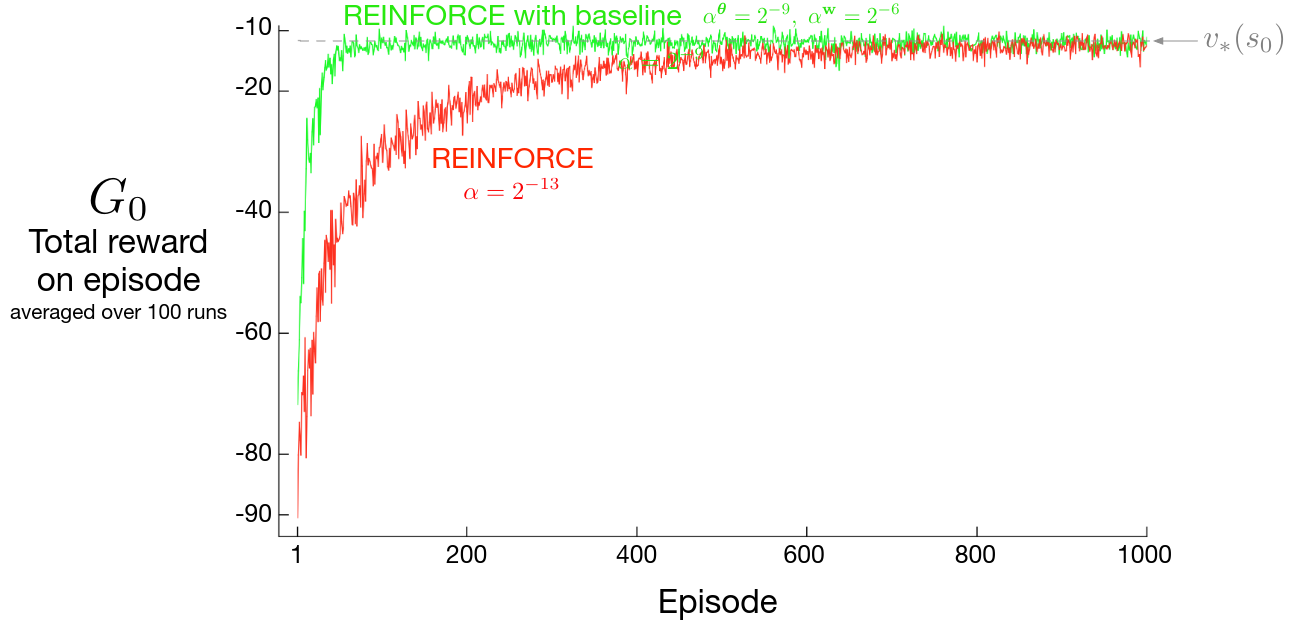
\includegraphics[width=\linewidth]{images/reinforce-comparison.png}
    \caption{Comparison of the REINFORCE and REINFORCE with baseline algorithms on the short-corridor gridworld, with the optimal step sizes indicated. The results show that the baseline algorithm outperforms the REINFORCE algorithm, reaching the best return in just 100 steps, while the REINFORCE algorithm takes roughly 1000 steps. Image taken from \cite{sutton-barto}.}
    \label{fig:reinforce-comparison}
\end{figure}

\section{Actor-Critic Methods}
The REINFORCE with baseline algorithm is unbiased, but it has a high variance and is therefore slow to converge. Additionally, it is challenging to extend it to continuous tasks. In order to address these issues, Actor-Critic methods merge policy gradient and bootstrapping by using the one-step return $G_{t:t+1}$ instead of the full return $G_t$ to update the policy.\\\\
More in detail, the policy parameter vector $\vect{\theta}$ is updated using policy gradient and TD-learning is used to update the value function $v_{\pi_{\theta}}(s; \vect{w})$. This adds a bias in the policy gradient update, but it also reduces variance and speeds up learning.\\
In particular, one-step actor-critic methods update the policy as following:
\begin{equation}
    \theta_{t+1} = \theta_t + \alpha (G_{t:t+1} - \hat{v}_{\pi_{\theta}}(S_t; \vect{w})) \frac{\nabla_{\theta} \pi_{\theta}(A_t|S_t)}{\pi_{\theta}(A_t|S_t)}
    \label{eq:one-step-actor-update}
\end{equation}
Which is similar to the REINFORCE with baseline update \eqref{eq:reinforce-with-baseline-update}, but uses the one-step return $G_{t:t+1} = R_{t+1} + \gamma \hat{v}(S_{t+1}; \vect{w})$ instead of the full return $G_t$ \eqref{return}.\\
At the same time, the value function parameters $\vect{w}$ are updated towards the bootstrapping target $G_{t:t+1}$:
\begin{equation}
    \vect{w}_{t+1} = \vect{w}_t + \alpha (G_{t:t+1} - \hat{v}_{\pi_{\theta}}(S_t; \vect{w})) \nabla_{\vect{w}} \hat{v}_{\pi_{\theta}}(S_t; \vect{w})
    \label{eq:one-step-critic-update}
\end{equation}
The actor-critic update can be generalized to $n$-step returns by simply replacing the one-step return $G_{t:t+1}$, with the $n$-step return $G_{t:t+n}$ \eqref{n-step-return} in equations \eqref{eq:one-step-actor-update} and \eqref{eq:one-step-critic-update}.\\

\section{Trust Region Policy Optimization}
Trust Region Policy Optimization (TRPO) \cite{schulman2015trust} is an actor-critic method that uses a trust region to constrain the policy update. The TRPO update tries to improve the policy as much as possible while satisfing a special constraint that says how much the old and updated policy are allowed to differ. TRPO fixes a major problem of vanilla policy gradient, where the policy update, even though it changes the parameters only slightly, can have dramatic effects on performance, thus a bad policy update can lead to performance collapse.\\\\
Mathematically, the TRPO update is defined as follows:
\begin{equation}
    \begin{split}
        \theta_{t+1} = & \arg\max_{\theta} \; L(\theta_t, \theta)\\
        & \; \text{s.t.} \; \bar D_{KL}(\pi_{\theta_t}, \pi_{\theta}) \leq \delta        
    \end{split}
    \label{eq:trpo-update}
\end{equation}
Where $L(\theta_t, \theta)$ is the surrogate advantage, $\delta$ is a trust region parameter and $\bar D_{KL}(\pi_{\theta_t}, \pi_{\theta})$ is the average KL-divergence across states between the old and new policy.\\
More in detail, $L(\theta_t, \theta)$ tells us how much better the new policy is according to data from the old policy
\begin{equation}
    L(\theta_t, \theta) = \underset{s, a \sim \pi_{\theta_t}}{\mathbb{E}} \left[ \frac{\pi_{\theta}(a|s)}{\pi_{\theta_t}(a|s)} A_{\pi_{\theta_t}}(s, a) \right]
    \label{eq:surrogate-advantage}
\end{equation}
Where $A_{\pi_{\theta_t}}(s, a)$ is the advantage function \eqref{advantage}, which measures how much better action $a$ is than the average action in state $s$, while the factor $\frac{\pi_{\theta}(a|s)}{\pi_{\theta_t}(a|s)}$ is the ratio of the probabilities of the new and old policy. So, if the new policy puts more weight on actions with higher advantage, then the surrogate advantage will be higher and the new policy will be better than the old one.\\
Whereas the constraint $\bar D_{KL}(\pi_{\theta_t}, \pi_{\theta})$ is the average KL-divergence across states between the old and new policy.
\begin{equation}
    \bar D_{KL}(\pi_{\theta_t} || \pi_{\theta}) = \underset{s \sim \pi_{\theta_t}}{\mathbb{E}} \left[ D_{KL}(\pi_{\theta_t}(\cdot|s) || \pi_{\theta}(\cdot|s)) \right]
    \label{eq:kl-divergence}
\end{equation}
The TRPO update in equation \eqref{eq:trpo-update} is a constrained optimization problem, which can be solved using a variety of methods. Here we will provide a simple solution by approximating the objective \eqref{eq:surrogate-advantage} to the first order and the constraint \eqref{eq:kl-divergence} to the second order.\\
\begin{equation}
    L(\theta_t, \theta) \approx g^T (\theta - \theta_t)
\end{equation}
\begin{equation}
    \bar D_{KL}(\pi_{\theta_t} || \pi_{\theta}) \approx \frac{1}{2} (\theta - \theta_t)^T H (\theta - \theta_t)
\end{equation}
The reason we are approximating the constraint to the second order is because the KL divergence has minima at $\theta = \theta_t$, so its gradient is zero.\\\\
With these approximations the TRPO update becomes:
\begin{equation}
    \begin{split}
        \theta_{t+1} = & \arg\max_{\theta} \; g^T (\theta - \theta_t)\\
        & \; \text{s.t.} \; \frac{1}{2} (\theta - \theta_t)^T H (\theta - \theta_t) \leq \delta        
    \end{split}
    \label{eq:trpo-update-approx}
\end{equation}
The solution to this optimization problem is on the boundary, because we are maximizing a linear function on a convex domain, so it can be solved exactly using the Lagrangian method, yielding the solution:
\begin{equation}
    \theta_{t+1} = \theta_t + \sqrt{\frac{2\delta}{g^T H^{-1} g}} H^{-1} g
    \label{eq:trpo-update-solution}
\end{equation}
Note that no learning rate is needed in the TRPO update, since the trust region parameter $\delta$ controls the size of the update.\\
A problem of the approximate update \eqref{eq:trpo-update-solution} is that the constraint \eqref{eq:kl-divergence} can be broken before reaching the boundary, to solve this problem we can use a backtracking line search to find the maximum step size that satisfies the constraint.\\
\begin{equation}
    \theta_{t+1} = \theta_t + \alpha^j \sqrt{\frac{2\delta}{g^T H^{-1} g}} H^{-1} g
    \label{eq:trpo-update-line-search}
\end{equation}
Where $\alpha \in (0, 1)$ is the backtracking coefficient and $j$ is the smallest integer such that constraint \eqref{eq:kl-divergence} is satisfied.\\

\section{Proximal Policy Optimization}
Proximal Policy Optimization (PPO) \cite{schulman2017proximal} tries to answer the same question as TRPO, how can we take the biggest policy improvement without having a performance collapse? The main difference between PPO and TRPO is that PPO solves the problem using a first order method, which is much simpler to implement and faster to train, as we don't need to compute the inverse Hessian-gradient product \eqref{eq:trpo-update-line-search}. There are two versions of PPO, PPO-penalty and PPO-clip. We will focus on PPO-clip, as it is the most popular one.\\\\

PPO updates the policy using the following equation:
\begin{equation}
    \theta_{t+1} = \arg\max_{\theta} \underset{s, a \sim \pi_{\theta_t}}{\mathbb{E}} \left[ L(s, a, \theta_t, \theta) \right]
    \label{eq:ppo-update}
\end{equation}
Where $L$ is defined as:
\begin{equation}
    \begin{split}
        L(s, a, \theta_t, \theta) = \min \bigg(& \frac{\pi_{\theta}(a|s)}{\pi_{\theta_t}(a|s)} A_{\pi_{\theta_t}}(s, a),\\
        & \; \text{clip}(\frac{\pi_{\theta}(a|s)}{\pi_{\theta_t}(a|s)}, 1 - \epsilon, 1 + \epsilon) A_{\pi_{\theta_t}}(s, a)\bigg)
    \end{split}
    \label{eq:ppo-update-clip}
\end{equation}
The objective function $L(s, a, \theta_t, \theta)$ in equation (\ref{eq:ppo-update-clip}) is defined as the minimum between two terms. The first term represents the surrogate advantage function and the second term is a clipped version of the policy ratio $\frac{\pi_{\theta}(a|s)}{\pi_{\theta_t}(a|s)}$, where $\epsilon$ is a small hyperparameter (typically set near 0.1) that determines the extent to which the policy can deviate from the previous policy. The purpose of the clipping is to prevent the policy from making too big of a change, which can lead to performance collapse. The clipping also ensures that the old policy data remains representative of the new policy if the policy ratio is significantly different from 1.
\begin{figure}[H]
    \centering
    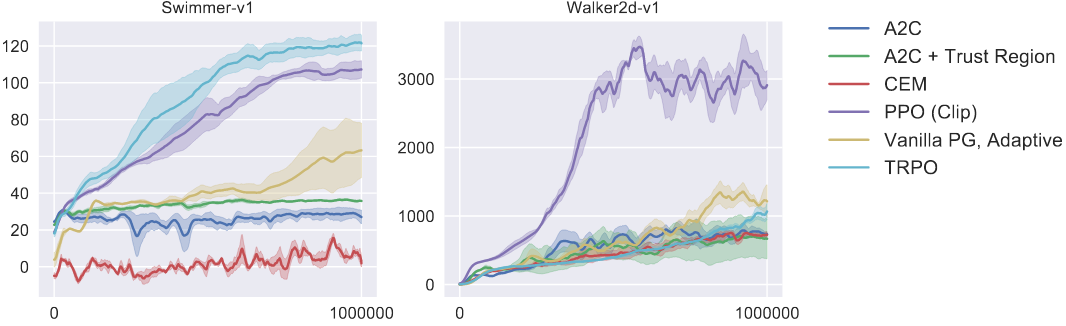
\includegraphics[width=\textwidth]{images/ppo-comparison.png}
    \caption{Comparison of several algorithms on two different environments. PPO exceeds the performance of TRPO and VPG. Image taken from \cite{schulman2017proximal}.}
    \label{fig:ppo-comparison}
\end{figure}

\section{Generalized Advantage Estimation}
In the previous two sections we focused on the policy update, leaving details on how we can compute and learn the advantage $A_{\pi_{\theta_t}}(s, a)$.\\
There are many estimators of the advantage, for example in vanilla policy gradient \eqref{eq:one-step-critic-update} we used $A_{\pi_{\theta_t}}(S_t, A_t) = G_{t:t+1} - V_{\pi_{\theta_t}}(S_t; \vect{w})$ which is the TD-error, while in REINFORCE we used the full return $G_t$ \ref{eq:reinforce-update}. In general, the policy gradient can be written in a more general way \cite{schulman2015high}:
\begin{equation}
    \nabla_\theta J = \mathbb{E} \left[ \sum_{t=0}^{\infty} \Psi_t \nabla_\theta \log \pi_{\theta}(A_t|S_t) \right]
\end{equation}
Where $\Psi_t$ can be any method of advantage estimation, like:
\begin{itemize}
    \item $R_{t+1} + \gamma V_{\pi_{\theta_t}}(S_{t+1}; \vect{w}) - V_{\pi_{\theta_t}}(S_{t+1}; \vect{w})$ One-step TD target.
    \item $Q_{\pi_{\theta_t}}(S_t, A_t)$ Action-value function.
    \item $\sum_{k=0}^{\infty} \gamma^k R_{t+k+1}$ Full return.
    \item $A_{\pi_{\theta_t}}(S_t, A_t)$ Advantage function.
\end{itemize}
It can be proven that among these estimators the advantage function is the lowest variance estimator \cite{greensmith2004variance}.\\\\
Another advantage estimation method that is used in practice is Generalized Advantage Estimation (GAE) \cite{schulman2015high}. GAE is a popular advantage estimation method that combines the strengths of both Monte Carlo and TD methods. The GAE advantage is expressed as:
\begin{equation}
    A_{t}^{\textrm{GAE}}(s, a) = \sum_{k=0}^{\infty} \gamma^k \lambda^k \delta_{t+k}
    \label{eq:gae-advantage}
\end{equation}
Where $\delta_{t+k}$ is the TD-error at time $t+k$ and $\lambda \in (0, 1)$ is a hyperparameter that determines the weight given to future TD-errors. In particular, if $\lambda = 0$ then $A_t^{\textrm{GAE}} = \delta_t$, while if $\lambda = 1$ then $A_t^{\textrm{GAE}} = G_t$. The $\lambda$ parameter thus makes a compromise between the bias and variance of the estimator, like the parameter $n$ does for $n$-step TD methods \ref{n-step-return}. Figure \ref{fig:gae-comparison} shows the performance of GAE with different values of $\lambda$.\\
Currently, GAE is used in all major reinforcement learning libraries, like CleanRL \cite{huang2022cleanrl}, Tianshou \cite{tianshou} and Stable Baselines3 \cite{stable-baselines3}.
\begin{figure}[H]
    \centering
    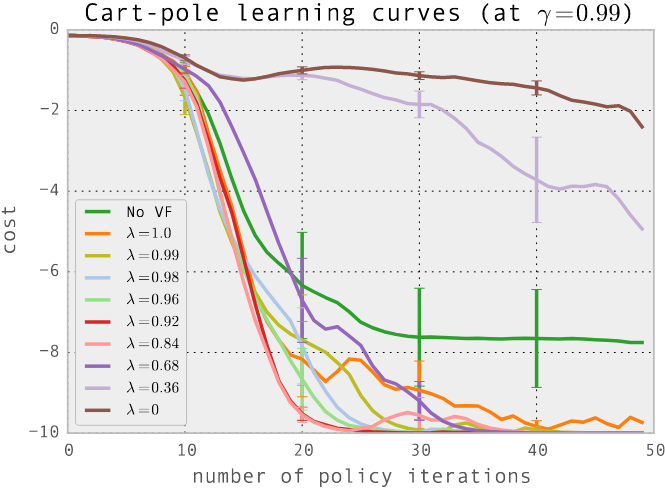
\includegraphics[width=0.7\textwidth]{images/gae-comparison.png}
    \caption{Comparison of GAE with various values of $\lambda$ in the Cart-pole environment using TRPO to learn the policy. We can see that $\lambda \in [0.9, 0.99]$ performs best. Image taken from \cite{schulman2015high}.}
    \label{fig:gae-comparison}
\end{figure}